\documentclass{standalone}
\usepackage{tikz}
\usetikzlibrary{arrows}

\begin{document}
	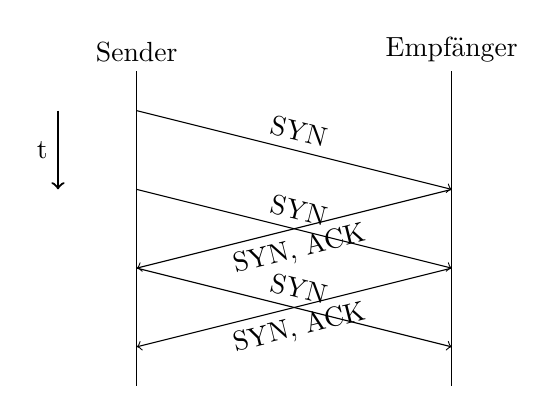
\begin{tikzpicture}
		\path[->, thick] (-1, -1) edge node[midway, left] {t} (-1, -2);
		
		\path[draw] (0, -0.5) -- node[above, pos=0] {Sender} (0, -4.5);
		\path[draw] (4, -0.5) -- node[above, pos=0] {Empfänger} (4, -4.5);
		
		\path[->] (0, -1) edge node[above, sloped] {SYN} (4, -2);
		\path[<-] (0, -3) edge node[below, sloped] {SYN, ACK} (4, -2);
		\path[->] (0, -2) edge node[above, sloped] {SYN} (4, -3);
		\path[<-] (0, -4) edge node[below, sloped] {SYN, ACK} (4, -3);
		\path[->] (0, -3) edge node[above, sloped] {SYN} (4, -4);
	\end{tikzpicture}
\end{document}